\begin{tikzpicture}
\begin{axis} [
     title={},
     width=\textwidth,
     height=.25\textheight,
     xlabel={\footnotesize \textbf{Visual Pattern}},
     ylabel={\footnotesize \textbf{Accuracy}},
     bar width = 4pt,
     ybar = .02cm,
     xmin=0.0, xmax=5,
     ymin=0.0, ymax=850,
     x tick label style={font=\tiny},
     y tick label style={font=\tiny},
     xtick={1,2,3,4},
     xticklabels={VQA - Fail, Grounding - Fail, Both - Fail, Both - Success},
     y label style={at={(axis description cs:0.05,.5)},anchor=south},
     ymajorgrids=false,
     xmajorgrids=false,
     legend style={
			at={(0.5,-0.35)},
			anchor=north,
			legend columns=5,
            }
] 

\addplot[color=blue!40, fill=blue, area legend] coordinates{(1, 525) (2, 232) (3, 417) (4, 264)};
\addplot[color=blue!40, fill=blue!60,  area legend] coordinates {(1, 173) (2, 409) (3, 756) (4, 100)};
\addplot[color=blue!40, fill=blue!30,  area legend] coordinates {(1, 593) (2, 36) (3, 660) (4, 149)};
\addplot[color=blue!40, fill=blue!10,  area legend] coordinates {(1, 821) (2, 1) (3, 615) (4, 1)};
\addplot[color=blue!40, fill=blue!2,  area legend] coordinates {(1, 48) (2, 105) (3, 136) (4, 11)};

\addplot[color=blue!40, fill=red!20,  area legend] coordinates {(1, 269) (2, 383) (3, 650) (4, 136)};
\addplot[color=blue!40, fill=red!60,  area legend] coordinates {(1, 292) (2, 325) (3, 724) (4, 97)};
\addplot[color=blue!40, fill=red,  area legend] coordinates {(1, 0) (2, 0) (3, 0) (4, 0)};

\legend{\textbf{OMG-Llava (7B)}, \textbf{Llava-G (7B)}, \textbf{LISA (7B)}, \textbf{GLaMM (7B)}, \textbf{GLaMM$\dagger$ (7B)}, \textbf{Llava (13B)}, \textbf{Llava (7B)}, \textbf{Cambrian (8B)}}

\end{axis}
\end{tikzpicture}